\documentclass[a4paper]{article}
\usepackage{amsmath,amssymb}
\usepackage{graphicx} % Required for inserting images
\usepackage{tikz}
\usepackage{hyperref}
\usepackage{cleveref}
\usepackage{pgfplots}
\usetikzlibrary{calc,arrows,shapes,positioning}
\usepackage{standalone}
\usepackage{subcaption}
\usepackage{booktabs}
\usepackage{siunitx} 
\usepackage{IAM_Lager}


\newtheorem{problem}{Problem}

\newcommand{\R}{\mathbb{R}}


\title{Optimization Methods for Sustainable Building Constructions}
\author{xxx}
\date{March 2026}

\begin{document}

\maketitle
\begin{abstract}

\end{abstract}


\tableofcontents
\clearpage
%%%%%%%%%%%%%%%%%%%%%%%%%%%%%%%%%%%%%%%%%%%%%%%%%%%%%%%%%%%%%%
\section{Parametric optimization of a timber girder}
\begin{figure}[htb]
    \centering
    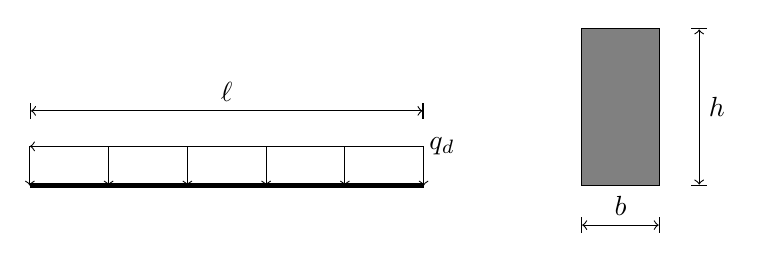
\begin{tikzpicture}
		\coordinate (A) at (0,0);
		\draw[ultra thick] (0,0) -- (5,0);
		\draw[|<->|] (0,0.95) -- ++(5,0.0) node[pos=.5,above]{$\ell$};
		\foreach \x in {0,1,2,3,4,5}{
		\draw[<-] (\x,0) -- ++(0,0.5); };
		\draw[<-] (0,0.5) -- ++(5.0,0) node[pos=0.99,right]{$q_d$};
		\Festlager{A};
		\Loslager{5,0};
		\draw[fill=gray] (7,0) rectangle ++(1,2);
		\draw[|<->|] (7,-0.5) -- ++(1,0) node[pos=.5,above]{$b$};
		\draw[|<->|] (8.5,0.) -- ++(0,2) node[pos=.5,right]{$h$};
	\end{tikzpicture}	
    \caption{Mechanical system and cross-section of the parametric optimization of a timber girder}
    \label{fig:timber}
\end{figure}
	 \begin{problem}\label{prob:timeber}
	     Given $\ell,\; q_d\in\R$. Find the optimal rectangular cross-section $(b,h)\in \mathbb R^2_+$ such that the used timber is minimized. Consider the bending, shear and deflection proofs.
    Furthermore, the width should not exceed $b_{max}\in\R_+$ and the height should not exceed $h_{max}\in\R_+$.
\end{problem}
A mathematical formulation of \Cref{prob:timeber} reads: Find $(b,h)\in \mathbb R^2$ such that
	\begin{equation*}
		A(b,h) = b h  \rightarrow min,
	\end{equation*}
	subjected to the inequality constraints
	\begin{align*}
		g_{bending}(b,h) \le 0, \qquad g_{shear}(b,h) \le 0, \qquad
		g_{SLS}(b,h) \le 0,
	\end{align*}
	and the box-constraints
	\begin{align*}
	0\le b \le b_{max},\quad 0\le h \le h_{max}.
	\end{align*}
Here, we assume that the mechanics of the proofs is
	\begin{align*}
		g_{bending}(b,h) &= \tfrac{M_{max}}{W_y(b,h)}- k_{crit}(b,h)f_{md}  &&\mbox{with} \quad M_{max} = \tfrac{q_d\ell^2}{8},\\
		g_{shear}(b,h) &= \tfrac{3}{2}\tfrac{Q_{max}}{A(b,h)} - f_{vd} &&\mbox{with} \quad Q_{max} = \tfrac{q_d\ell}{2},\\
		g_{SLS}(b,h) &= w_{max} - w_{adm}&&\mbox{with} \quad w_{max} = \tfrac{5}{384} \tfrac{ q_d  \ell^4}{E_{mean} Iy(b,h)}.
	\end{align*}
According to (Seite B.3/80) the overturning coefficient $k_{crit}$ is calculated by 
	\begin{align*}
		k_{crit}(b,h) = \begin{cases}
			1 \quad &\text{if \quad} \lambda_{rel,m} \leq 0.75\\
			1.56-0.75 \,\lambda_{rel,m} \quad &\text{if \quad} 0.75 < \lambda_{rel,m} \leq 1.4\\
			\frac{1}{\lambda_{rel,m}^2} \quad &\text{if \quad} 1.4 < \lambda_{rel,m},
		\end{cases}
	\end{align*}
where the relative lateral-torsional slenderness is
\begin{equation*}
	\lambda_{rel,m} = \sqrt{\frac{f_{m,k}}{\sigma_{m,crit}}} \qquad \mbox{with} \quad \sigma_{m,crit} = \frac{\pi\sqrt{E_{0.05}I_zG_{0.05}I_{tor}}}{\ell_\text{eff}{W_y}}.
\end{equation*}    
%%%%%%%%%%%%%%%%%%%%%%%%%%%%%%%%%%%%%%%%%%%%%%%%%%%%%%%%%%%%%%

\end{document}
